
\documentclass[aspectratio=169]{beamer}
\usetheme{metropolis}
 \usepackage[utf8]{inputenc}
 \usepackage[french]{babel}
 %\usepackage[T1]{fontenc}


\usepackage{listings}

 \usepackage{hyperref}
\hypersetup{
    colorlinks=true,
    linkcolor=black,
    filecolor=magenta,
    urlcolor=cyan,
}

 \lstset{
  frame=tb,
  language=c++,
  aboveskip=3mm,
  belowskip=3mm,
  showstringspaces=false,
  columns=flexible,
  basicstyle={\footnotesize\ttfamily},
  numbers=none,
  numberstyle=\tiny\color{gray},
  keywordstyle=\color{blue},
  commentstyle=\color{orange},
  stringstyle=\color{purple},
  breaklines=true,
  breakatwhitespace=true,
  tabsize=4
}

\usepackage{mathtools}

\newcommand{\bfa}[0]{\boldsymbol{a}}
\newcommand{\bfb}[0]{\boldsymbol{b}}
\newcommand{\bfc}[0]{\boldsymbol{c}}
\newcommand{\bfd}[0]{\boldsymbol{d}}
\newcommand{\bff}[0]{\boldsymbol{f}}
\newcommand{\bfg}[0]{\boldsymbol{g}}
\newcommand{\bfh}[0]{\boldsymbol{h}}
\newcommand{\bfI}[0]{\boldsymbol{I}}
\newcommand{\bfj}[0]{\boldsymbol{j}}
\newcommand{\bfk}[0]{\boldsymbol{k}}
\newcommand{\bfl}[0]{\boldsymbol{l}}
\newcommand{\bfm}[0]{\boldsymbol{m}}
\newcommand{\bfn}[0]{\boldsymbol{n}}
\newcommand{\bfo}[0]{\boldsymbol{o}}
\newcommand{\bfq}[0]{\boldsymbol{q}}
\newcommand{\bfr}[0]{\boldsymbol{r}}
\newcommand{\bfs}[0]{\boldsymbol{s}}
\newcommand{\bft}[0]{\boldsymbol{t}}
\newcommand{\bfu}[0]{\boldsymbol{u}}
\newcommand{\bfv}[0]{\boldsymbol{v}}
\newcommand{\bfw}[0]{\boldsymbol{w}}
\newcommand{\bfx}[0]{\boldsymbol{x}}
\newcommand{\bfX}[0]{\boldsymbol{X}}
\newcommand{\bfy}[0]{\boldsymbol{y}}
\newcommand{\bfz}[0]{\boldsymbol{z}}
\newcommand{\bfe}[0]{\boldsymbol{e}}
\newcommand{\bfi}[0]{\boldsymbol{i}}
\newcommand{\bfp}[0]{\boldsymbol{p}}
%
 %\usepackage{multimedia}
%\begin{document}
%\movie[height = 0.6 \textwidth,width = 1.0 \textwidth]{}{animation.mpg}


%Information to be included in the title page:
%\title{Sample title}
%\author{Anonymous}
%\institute{ShareLaTeX}
%\date{2014}


 \AtBeginSection[]
{
  \begin{frame}
    \frametitle{Table des matières}
    \tableofcontents[currentsection]
  \end{frame}
}

\AtBeginSubsection[]
{
 \begin{frame}
   \frametitle{Table des matières}
   \tableofcontents[currentsubsection]
 \end{frame}
}

\begin{document}
\setbeamertemplate{caption}{\raggedright\insertcaption\par}

\title[Introduction à Gmsh]
{Introduction à Gmsh}

\subtitle{}

\author[Arthur Bawin]
{Arthur Bawin}

% \institute[] % (optional)
% {
%   \inst{1}%
%   Université catholique de Louvain
%   \and
%   \inst{2}%
%   École Polytechnique de Montréal
% }

\date[EPM 2021] % (optional)
{École Polytechnique de Montréal, 17 septembre 2021}

%\logo{\includegraphics[height=1.5cm]{lion-logo.png}}
\frame{\titlepage}

\begin{frame}
\frametitle{Licence}
Cette présentation \textit{open source} est sous License MIT. Le code source et les figures de la présentation sont disponibles sur Github : \url{https://github.com/arthurbawin/presentationGmshSept2021} \\
~\\
%\;\\
\textbf{ Copyright 2021 Arthur Bawin}

\footnotesize{Permission is hereby granted, free of charge, to any person obtaining a copy of this software and associated documentation files (the "Software"), to deal in the Software without restriction, including without limitation the rights to use, copy, modify, merge, publish, distribute, sublicense, and/or sell copies of the Software, and to permit persons to whom the Software is furnished to do so, subject to the following conditions:
The above copyright notice and this permission notice shall be included in all copies or substantial portions of the Software.}
\end{frame}

\begin{frame}
\frametitle{Table des matières}
\tableofcontents
\end{frame}

\section{Qu'est-ce que Gmsh ?}
\begin{frame}[fragile]
\frametitle{Gmsh c'est...}
\begin{itemize}
  \item ... \textbf{un outil basique de modélisation géométrique}
  \item ... \textbf{un générateur de maillages} 1D, 2D et 3D
  \begin{itemize}
    \item simpliciaux (triangles/tétraèdres) et outils pour maillages quadrangles/hexaèdres
    \item courbes sur les frontières CAD
  \end{itemize}
  \item ... une interface vers des solveurs externes (via ONELAB)
  \item ... un outil de visualisation et de post-traitement
  \item ... un logiciel libre, gratuit et open-source en développement actif
\end{itemize}
Utilisation :
\begin{itemize}
  \item \textbf{via l'interface graphique} (mode interactif)
  \item \textbf{en ligne de commande} (mode non-interactif)
  \item \textbf{comme bibliothèque via l'API} (C/C++, Python, Julia)
\end{itemize}

\end{frame}

\section{Maillage d'une géométrie 2D...}
\begin{frame}[fragile]
\frametitle{Un exemple de géométrie 2D}
\only<1>{Considérons le problème suivant :}
\only<2>{Étape par étape :}

\begin{columns}
  \begin{column}{0.7\textwidth}
    \begin{figure}[h!]
      \centering
      \begin{tikzpicture}[scale=0.8]
        \only<1>{
          \node (O) at (6,2) {$\Omega$};
          \node[left] (G1) at (0,2) {$~~\Gamma_1~~~$};
          \node[below] (G21) at (5,0) {$\Gamma_2$};
          \node[above] (G22) at (5,4) {$\Gamma_2$};
          \node[right] (G3)  at (10,2) {$\Gamma_3$};
          \node[above right] (G4)  at (3,2) {$\Gamma_4$};
        }
        \draw[draw=black, thick] (0,0) rectangle ++(10,4);
        \draw[thick] (3,2) arc[start angle=0, end angle=360,radius=0.5cm];
        \only<2>{
          \draw[fill=yellow!20] (0,0) rectangle ++(10,4);
          \draw[draw=red, very thick] (0,0) -- (10,0);
          \draw[draw=red, very thick] (0,4) -- (10,4);
          \draw[draw=green, very thick] (0,0) -- (0,4);
          \draw[draw=blue, very thick] (10,0) -- (10,4);
          \node (O) at (6,2) {Surface};
          \node[left] (G1) at (0,2) {Entrée};
          \node[below] (G21) at (5,0) {Bord};
          \node[above] (G22) at (5,4) {Bord};
          \node[right] (G3)  at (10,2) {Sortie};
          \node[above right] (G4)  at (3,2) {Cylindre};
          \draw[draw = orange, very thick, fill=white] (3,2) arc[start angle=0, end angle=360,radius=0.5cm];
        }
      \end{tikzpicture}
    \end{figure}
  \end{column}
  \hspace{0.5cm}
  \begin{column}{0.4\textwidth}
    \only<1>{
      \begin{align*}
        \nabla \cdot \bfu &= 0\\
        \frac{\partial \bfu}{\partial t} + (\bfu \cdot \nabla)\,\bfu &= -\frac{1}{\rho}\nabla p + \nu \Delta \bfu
      \end{align*}
      }
    \only<2>{
    \footnotesize
      \begin{enumerate}
        \item Créer les \textbf{entités géométriques} : points, courbes, surfaces, volumes
        \item Définir les \textbf{entités physiques} : groupes d'entités géométriques
        \item Spécifier la \textbf{taille des éléments}
        \item Générer le \textbf{maillage}
      \end{enumerate}
    }
  \end{column}
\end{columns}
\end{frame}

\begin{frame}[fragile]
\frametitle{Modélisation géométrique}
\footnotesize
  \begin{itemize}
    \item \textbf{Boundary Representation (B-REP)}: volume $\xrightarrow{\partial}$ surfaces $\xrightarrow{\partial}$ courbes $\xrightarrow{\partial}$ points
    \item Constructive Solid Geometry (CSG) : opérations booléennes sur des volumes
  \end{itemize}
  Ici, nous allons construire une géométrie à l'aide de sa B-REP (bottom-up)
  \begin{columns}
    \begin{column}{0.5\textwidth}
      \begin{figure}
        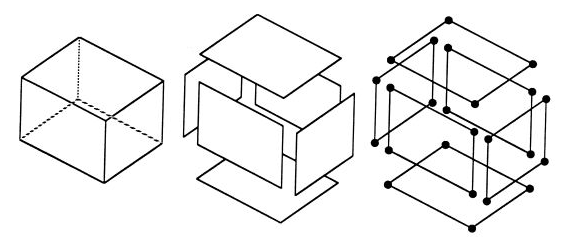
\includegraphics[width=0.8\textwidth]{figures/brep.png}
        \caption{B-REP \footnotemark[1]}
      \end{figure}
    \end{column}
    \begin{column}{0.5\textwidth}
      \begin{figure}
        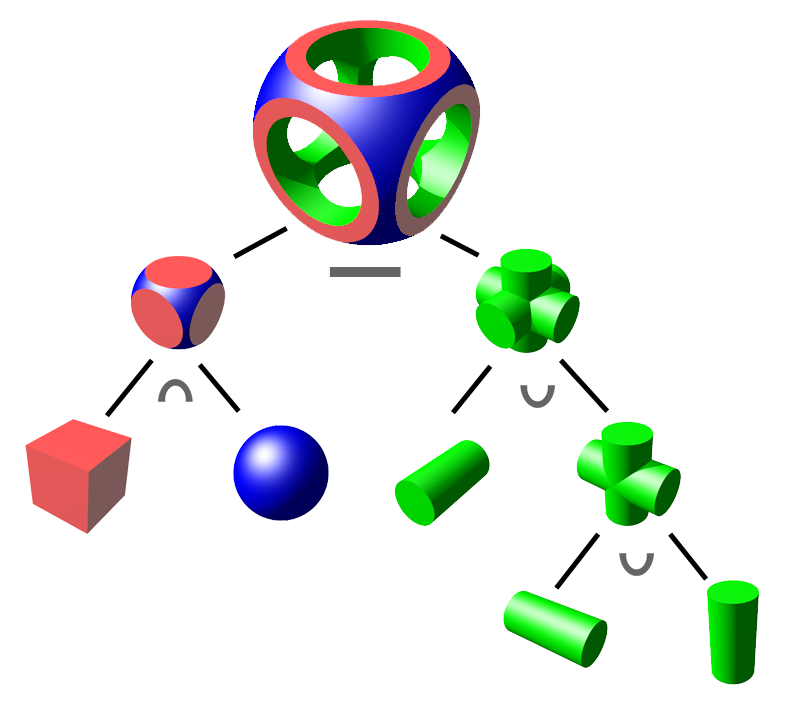
\includegraphics[width=0.65\textwidth]{figures/csg.png}
        \caption{CSG \footnotemark[2]}
      \end{figure}
    \end{column}
  \end{columns}
  \vspace{-0.4cm}
\footnotetext[1]{\tiny\url{https://ieda.ust.hk/dfaculty/ajay/courses/ieem575/lecs/cad_1/lecCAD1.html}}
\footnotetext[2]{\tiny\url{https://en.wikipedia.org/wiki/Constructive_solid_geometry}}
\end{frame}

\subsection{... à l'aide de l'interface graphique}
\begin{frame}[fragile]
\frametitle{Créer la géométrie dans l'interface graphique}
0 : Set geometry kernel $>$ OpenCASCADE
\begin{columns}
  \begin{column}{0.5\textwidth}

    \begin{figure}
      \centering
      \begin{tikzpicture}
        \node[anchor=south west,inner sep=0] (image) at (0,0)
        {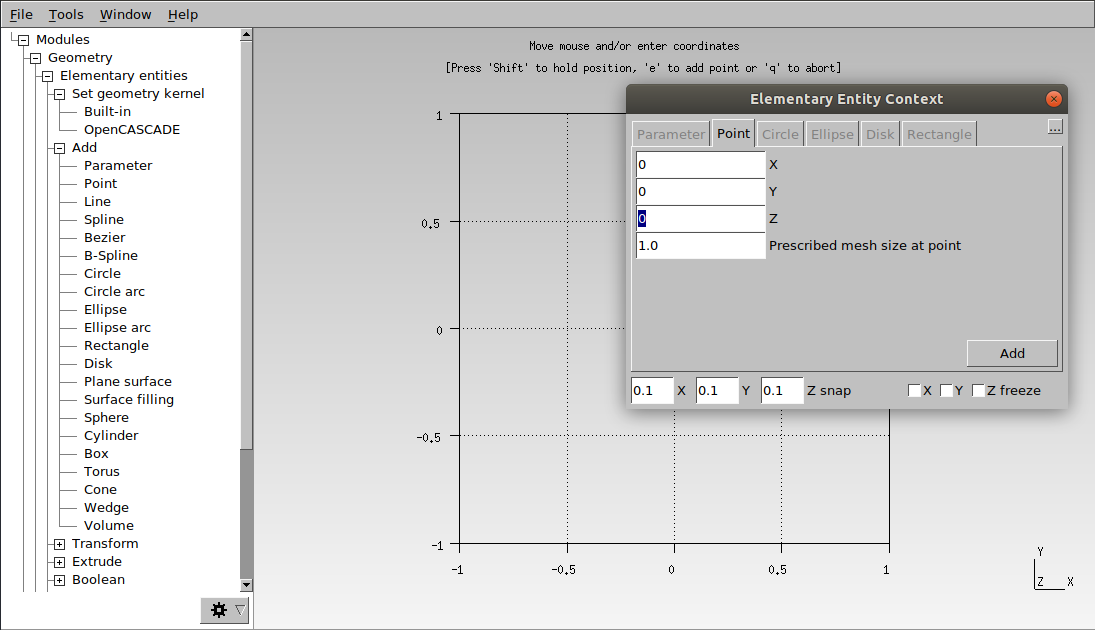
\includegraphics[width=\linewidth]{figures/points.png}};
        \begin{scope}[x={(image.south east)},y={(image.north west)}]
          \draw[draw=orange, thick] (0.07,0.78) rectangle ++(0.1,0.03);
          \draw[draw=orange, thick] (0.07,0.69) rectangle ++(0.045,0.035);
        \end{scope}
      \end{tikzpicture}
      \caption{1: Points (0,0), (10,0), (10,4), (0,4)}
    \end{figure}

  \end{column}
  \begin{column}{0.5\textwidth}
    \begin{figure}
      \centering
      \begin{tikzpicture}
        \node[anchor=south west,inner sep=0] (image) at (0,0)
        {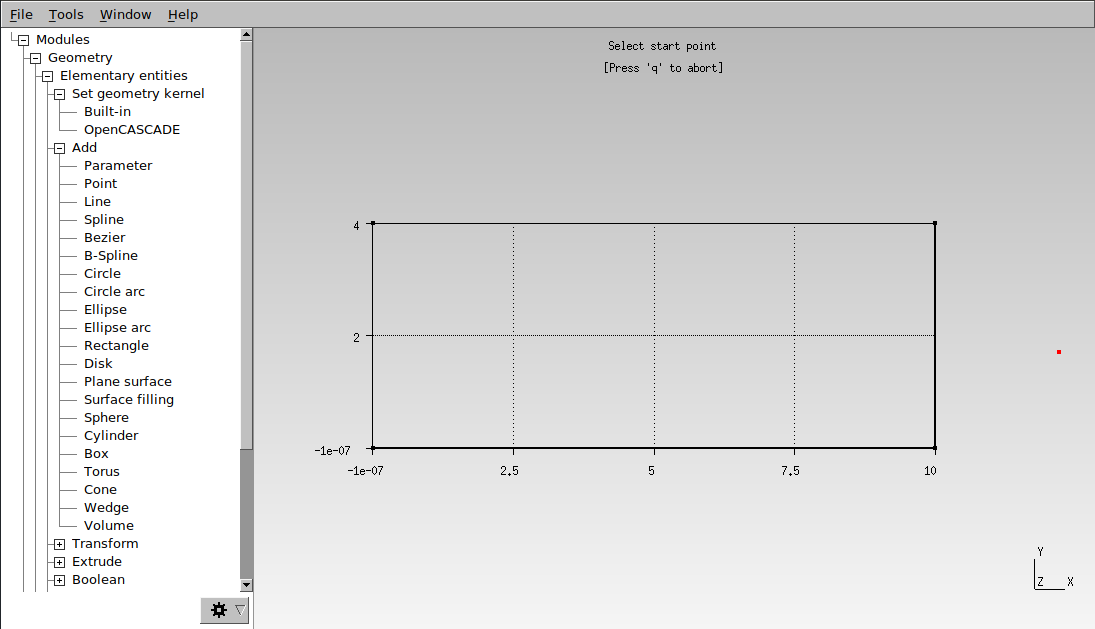
\includegraphics[width=\linewidth]{figures/lignes.png}};
        \begin{scope}[x={(image.south east)},y={(image.north west)}]
          \draw[draw=orange, thick] (0.07,0.663) rectangle ++(0.045,0.035);
        \end{scope}
      \end{tikzpicture}
      \caption{2: Lignes}
    \end{figure}
  \end{column}
\end{columns}

NB : La taille caractéristique doit être spécifiée à chaque point (1.0 par défaut)

\end{frame}

\begin{frame}[fragile]
\frametitle{Créer la géométrie dans l'interface graphique}
\begin{columns}
  \begin{column}{0.5\textwidth}
    \begin{figure}
      \centering
      \begin{tikzpicture}
        \node[anchor=south west,inner sep=0] (image) at (0,0)
        {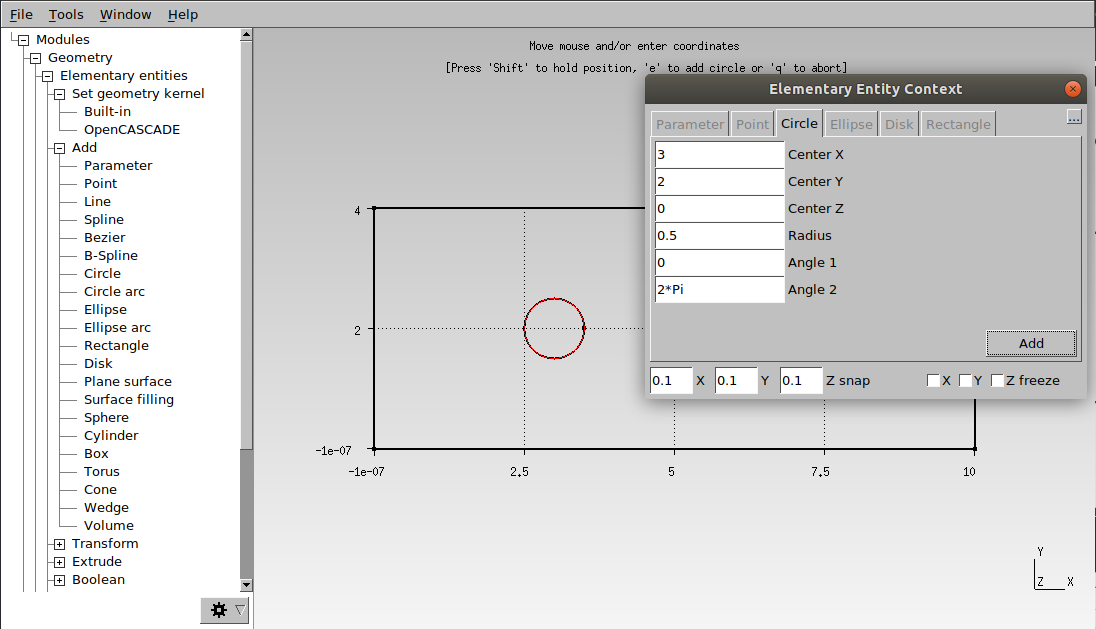
\includegraphics[width=\linewidth]{figures/cercle.png}};
        \begin{scope}[x={(image.south east)},y={(image.north west)}]
          \draw[draw=orange, thick] (0.07,0.55) rectangle ++(0.05,0.035);
        \end{scope}
      \end{tikzpicture}
      \caption{3: Cercle en (3,2)}
    \end{figure}
  \end{column}
  \begin{column}{0.5\textwidth}
    \begin{figure}
      \centering
      \begin{tikzpicture}
        \node[anchor=south west,inner sep=0] (image) at (0,0)
        {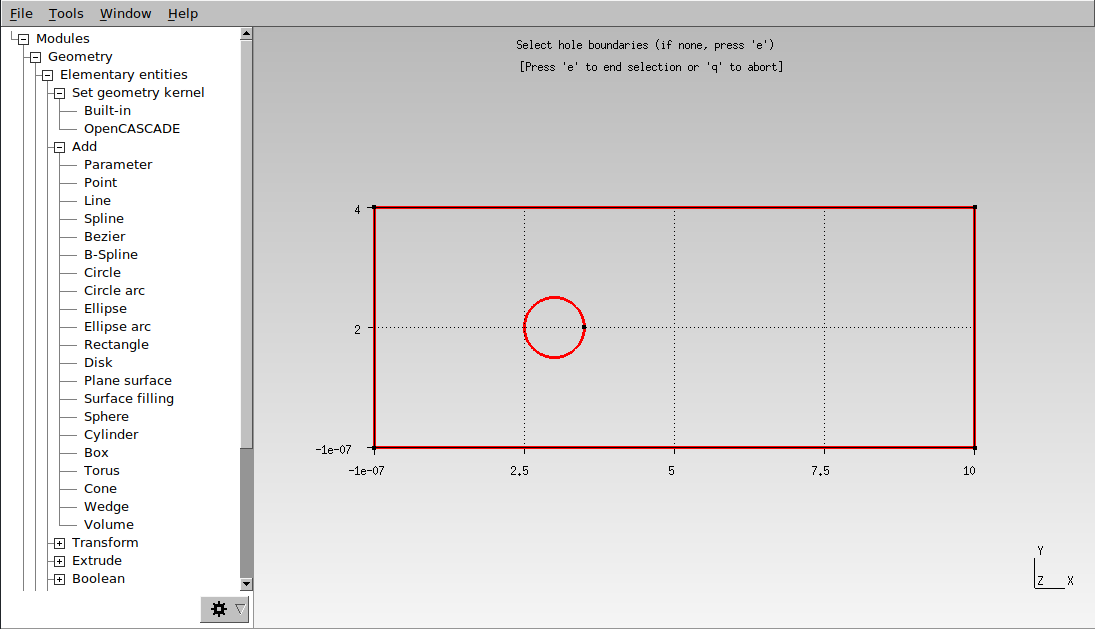
\includegraphics[width=\linewidth]{figures/surface.png}};
        \begin{scope}[x={(image.south east)},y={(image.north west)}]
          \draw[draw=orange, thick] (0.07,0.38) rectangle ++(0.095,0.035);
        \end{scope}
      \end{tikzpicture}
      \caption{4: Surface = Lignes (frontière) - Cercle (trou)}
    \end{figure}
  \end{column}
\end{columns}
\footnotesize
Ensuite (pas illustré ici : plus facile de passer par un script .geo) :
\begin{enumerate}
  \item[2.] Définir les entités physiques (groupes nommés d'entités géométriques)
  \item[3.] Spécifier éventuellement la taille grâce à un champ de taille
  \item[4.] Générer le maillage
\end{enumerate}

\end{frame}

\subsection{... en ligne de commande}

\begin{frame}[fragile]
\frametitle{Script .geo et syntaxe Gmsh}
\begin{itemize}
  \item Deux types de variables : \textit{real} (expr) et \textit{string} (char-expr)
  \item Ci-dessous, le type par défaut des arguments est "expr"
  \item \texttt{(expr)} désigne une nouvelle entité et \texttt{\{expr\}} réfère à une entité existante
  \item Entités géométriques de même dimension doivent avoir des \textit{tags} ($>0$) différents
\end{itemize}
\begin{lstlisting}[language=c++]
  // Creer un point
  Point(tag) = {x, y, z, lc = 1.0};
  // Creer une ligne/courbe
  Line(tag) = {tagBegin, tagEnd};
  Bezier(tag) = {expr-list controlPoints};
  BSpline(tag) = {expr-list controlPoints};
  Circle(tag) = {xc, yc, zc, r, beginAngle, endAngle};
  ...
  // Boucle orientee (!) de courbes : permet de definir une surface
  Curve Loop(tag) = {expr-list curveTags}; // Utiliser des signes "-" au besoin
\end{lstlisting}
\end{frame}

\begin{frame}[fragile]
\frametitle{Script .geo et syntaxe Gmsh}
\begin{lstlisting}[language=c++]
  // Creer une surface
  Plane Surface(tag) = {boundaryCurveLoopTag, expr-list holesCurveLoopTags = null};
  Surface(tag) = {expr-list curveLoopTags};
  Rectangle(tag) = {xllc, yllc, zllc, width, height}; // llc = lower-left corner
  Disk(tag) = {xc, yc, zc, r};
  ...
  // Boucle orientee de surfaces : permet de definir un volume
  Surface Loop(tag) = {expr-list surfaceTags};

  // Creer un volume
  Volume(tag) = {boundarySurfLoopTag, expr-list holesSurfLoopTags = null};
  Sphere(tag) = {xc, yc, zc, r};
  Box(tag) = {xllc, yllc, zllc, dx, dy, dz};
  Cylinder(tag) = {xc, yc, zc, xa, ya, za, r}; // center and axis
  Torus(tag) = {xc, yc, zc, r1, r2};
  ...
\end{lstlisting}
\end{frame}

\begin{frame}[fragile]
\frametitle{Script .geo et syntaxe Gmsh : entités physiques}
\begin{lstlisting}[language=c++]
  // Definir des entites physiques : groupes nommes d'entites geometriques
  Physical Point(tag) = {expr-list pointTags};
  Physical Point(char-expr name) = {expr-list pointTags};
  Physical Point(char-expr name) += {expr-list pointTags}; // incrementation


  Physical Curve(tag) = {expr-list curveTags};
  Physical Curve(char-expr name) = {expr-list curveTags};


  Physical Surface(tag) = {expr-list surfTags};
  Physical Surface(char-expr name) = {expr-list surfTags};


  Physical Volume(tag) = {expr-list volumeTags};
  Physical Volume(char-expr name) = {expr-list volumeTags};
\end{lstlisting}
\end{frame}

\begin{frame}[fragile]
\frametitle{Créer la géométrie dans un script foo.geo \hfill T1}
\begin{lstlisting}[frame=none,aboveskip=1mm]
// Le noyau OpenCASCADE est requis pour la fonction Circle
SetFactory("OpenCASCADE");
// Les coordonnees des coins et du centre
xmin = 0; xmax = 10;
ymin = 0; ymax = 4;
xc = 3; yc = 2; r = 0.5;
// La taille de maille (Characteristic Length) definie aux points
lc = 0.2;
// Les 4 coins
Point(1) = {xmin, ymin, 0, lc}; Point(2) = {xmax, ymin, 0, lc};
Point(3) = {xmax, ymax, 0, lc}; Point(4) = {xmin, ymax, 0, lc};
// Courbes orientees
Line(1) = {1,2};
Line(2) = {2,3};
Line(3) = {3,4};
Line(4) = {4,1}; // Attention a l'orientation
Circle(5) = {xc, yc, 0, r, 0, 2*Pi};
\end{lstlisting}
\end{frame}

\begin{frame}[fragile]
\frametitle{Créer la géométrie dans un script foo.geo \hfill T1}
\begin{lstlisting}[aboveskip=0.5mm,frame=none,escapechar=ß]
/* Le Point 5 a ete ajoute par Circle
Modifions sa taille de maille avec MeshSizeß\footnotemark[1]ß { expr-list } = expr */
MeshSize {5} = 0.01;
// newp retourne le prochain tag de Point disponible (newl, news, newv, newll, ...)
p5 = newp; Point(p5) = {1,1,0,lc}; // pas utilise ici

Curve Loop(1) = {1,2,3,4}; // Rectangle : frontiere de la surface
Curve Loop(2) = {5};          // Cercle : trou dans la surface
Plane Surface(1) = {1,2};

// Entites physiques (groupes nommes)
Physical Curve("Entree") = {4}; // -4 inverse la numerotation des elements
Physical Curve("Bord") = {1,3};
Physical Curve("Sortie") = {2};
Physical Curve("Cylindre") = {5};
Physical Surface("Surface") = {1};
\end{lstlisting}
\footnotetext[1]{Anciennement Characteristic Length}
\end{frame}

\begin{frame}[fragile]
\frametitle{Quick check \hfill T1}
\begin{lstlisting}[belowskip=1mm]
gmsh foo.geo
\end{lstlisting}
Cocher dans Tools $\rightarrow$ Options $\rightarrow$ Geometry $\rightarrow$ Visibility
  \begin{figure}
    \centering
    \begin{tikzpicture}
      \node[anchor=south west,inner sep=0] (image) at (0,0)
      {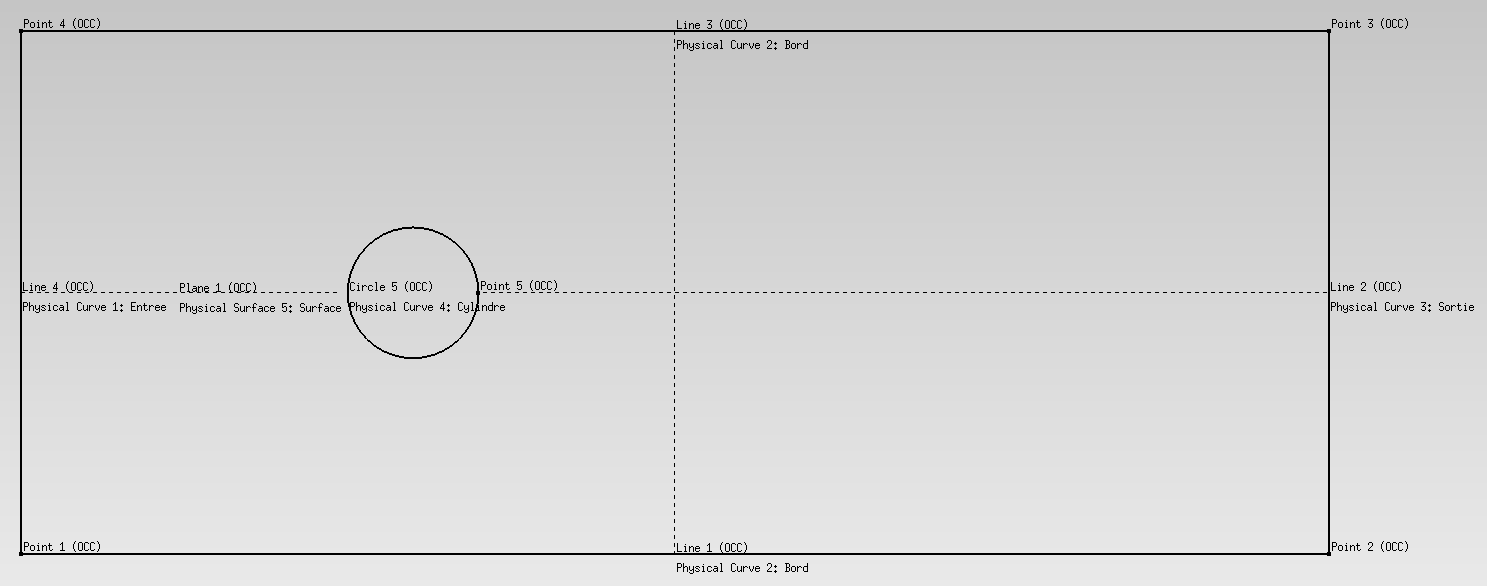
\includegraphics[width=\linewidth]{figures/geometrie.png}};
      \begin{scope}[x={(image.south east)},y={(image.north west)}]
        \draw[draw=orange, thick] (0.232,0.46) rectangle ++(0.11,0.035);
        \draw[draw=red, thick] (0.45,0.015) rectangle ++(0.097,0.035);
        \draw[draw=red, thick] (0.45,0.905) rectangle ++(0.097,0.035);
        \draw[draw=green, thick] (0.01,0.46) rectangle ++(0.105,0.035);
        \draw[draw=yellow, thick] (0.117,0.46) rectangle ++(0.113,0.035);
        \draw[draw=blue, thick] (0.89,0.46) rectangle ++(0.105,0.035);
      \end{scope}
    \end{tikzpicture}
  \end{figure}
\end{frame}

\begin{frame}[fragile]
\frametitle{Entités géométriques vs entités physiques}

\end{frame}

\begin{frame}[fragile]
\frametitle{Spécifier la taille des éléments}
\footnotesize
La taille de maille isotrope $h(\mathbf{x})$ est déterminée par :
  \begin{itemize}
    \item taille $h_1$ aux \textbf{Points} interpolée sur entités de dimensions supérieures : \texttt{MeshSizeFromPoints}
    \item taille $h_2$ calculée à partir de la \textbf{courbure du CAD} : \texttt{MeshSizeFromCurvature}
    \item un \textbf{champ de taille} $h_3$ défini à l'aide des champs Gmsh (\texttt{Fields})
    \item un \textbf{champ de taille externe} $h_4$ défini via l'API : \texttt{gmsh::model::mesh::setSizeCallback}
  \end{itemize}
  La taille est ensuite contrainte par :
  \begin{equation*}
    h(\mathbf{x}) = \texttt{MeshSizeFactor}~*~\max\biggr( \texttt{MeshSizeMin}, \min\left( h_1, h_2, h_3, h_4, \texttt{MeshSizeMax}\right) \biggr)
  \end{equation*}
  Si la taille est prescrite par un \textbf{champ}, utile de spécifier :
  \begin{lstlisting}[belowskip=0.5mm]
  Mesh.MeshSizeFromPoints = 0;
  Mesh.MeshSizeFromCurvature = 0;
  Mesh.MeshSizeExtendFromBoundary = 0;
  \end{lstlisting}
  pour éviter des conflits entre la taille prescrite par le champ et la taille prescrite sur les bords
\end{frame}

\begin{frame}[fragile]
\frametitle{Champs de taille \hfill T10}
\begin{columns}
  \begin{column}{0.65\textwidth}
    \footnotesize
    \textbf{Distance} : Calcule la distance à un point, une courbe ou une surface. Utilisé conjointement avec d'autres champs, comme Threshold ou MathEval.
    \begin{lstlisting}[frame=none,aboveskip=2mm,belowskip=1mm]
    Field[0] = Distance;
    Field[0].PointsList = {1};
    Field[0].CurvesList = {3};
    Field[0].NumPointsPerCurve = 100; // discretisation
    \end{lstlisting}
    % \vspace{0.6cm}
    \textbf{Threshold} :
    \vspace{-0.6cm}
    \begin{equation*}
      f(\mathbf{x}) =
        \begin{cases}
          \texttt{SizeMin} & \text{si } \texttt{Field[InField]} \leq \texttt{DistMin}\\
          \texttt{SizeMax} & \text{si } \texttt{Field[InField]} \geq \texttt{DistMax}\\
          \text{interpolation} & \text{sinon}
        \end{cases}
    \end{equation*}
    \begin{lstlisting}[frame=none,aboveskip=0mm,belowskip=0mm,escapechar=ß]
    Field[1] = Threshold;
    Field[1].InField = 0;
    Field[1].SizeMin = lc / 30; Field[1].SizeMax = lc;
    Field[1].DistMin = 0.15; ß~~ß Field[1].DistMax = 1.5;
    \end{lstlisting}
  \end{column}
  \begin{column}{0.35\textwidth}
    \vspace{1cm}
    \begin{tikzpicture}[]
      \node[below right] (P1) at (0,0) {P1};
      \node[above] (C3) at (2.5,2) {C3};
      \draw[draw=black, thick] (0,0) rectangle ++(5,2);
      \draw[draw=black, dashed] (0,1.5) -- ++(5,0);
      \draw[draw=black, dashed] (0,1.9) -- ++(5,0);
      \draw[thick] (1.5,1) arc[start angle=0, end angle=360,radius=0.25cm];
      \draw[dashed] (0.5,0) arc[start angle=0, end angle=90,radius=0.5cm];
      \draw[dashed] (0.1,0) arc[start angle=0, end angle=90,radius=0.1cm];
    \end{tikzpicture}
    \begin{figure}
      \text{~~~}
      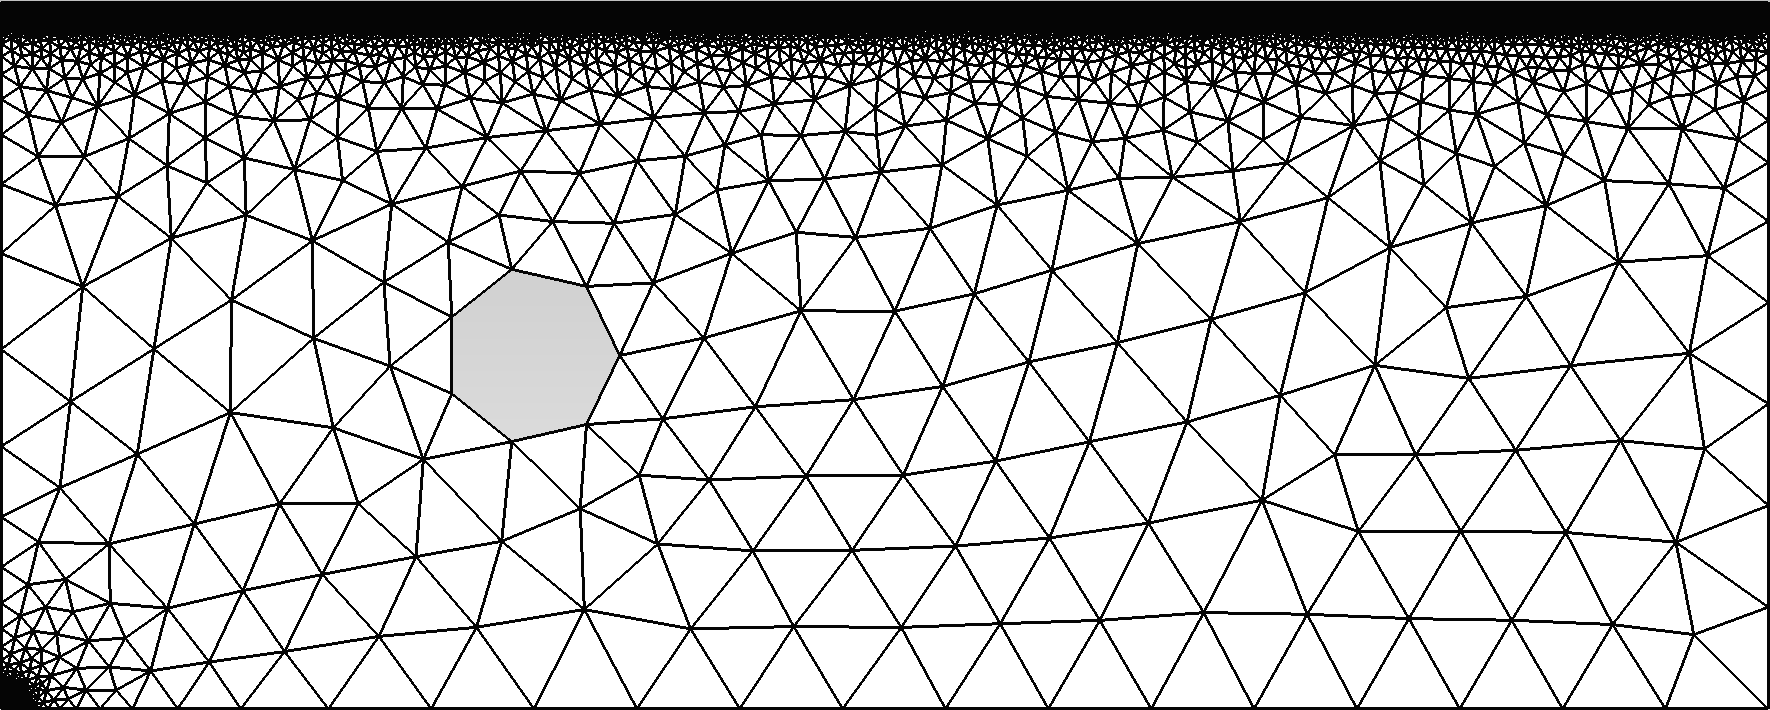
\includegraphics[width=1.02\textwidth]{figures/thresholdBW.png}
      \caption{}
      \label{}
    \end{figure}
  \end{column}
\end{columns}
\end{frame}

\begin{frame}[fragile]
\frametitle{Champs de taille \hfill T10}
\begin{columns}
  \begin{column}{0.65\textwidth}
    \footnotesize
    \textbf{MathEval} : Évalue l'expression fournie dans une chaîne de caractères. Supporte \texttt{F0, F1}, ... (référence aux champs), \texttt{x, y, z}, fonctions built-in (\texttt{Abs, Cos, Sin, Exp, ...}).
    \begin{lstlisting}[frame=none,aboveskip=2mm,belowskip=1mm]
    Field[2] = MathEval;
    Field[2].F = "0.05 + Abs(Cos(2*pi*x/5))/5";
    \end{lstlisting}
    À partir d'un autre champ :
    \begin{lstlisting}[frame=none,aboveskip=0mm,belowskip=3mm,escapechar=ß]
    Field[3] = MathEval;
    Field[3].F = "0.05 + F0^2"; // avec Distance
    \end{lstlisting}
    \textbf{Min} : Prend le minimum d'une liste de champs.
    \begin{lstlisting}[frame=none,aboveskip=2mm,belowskip=1mm]
    Field[4] = Min;
    Field[4].FieldsList = {1,2};
    \end{lstlisting}
  \end{column}
  \begin{column}{0.35\textwidth}
    \vspace{0.4cm}
    \begin{figure}
      \text{~~~}
      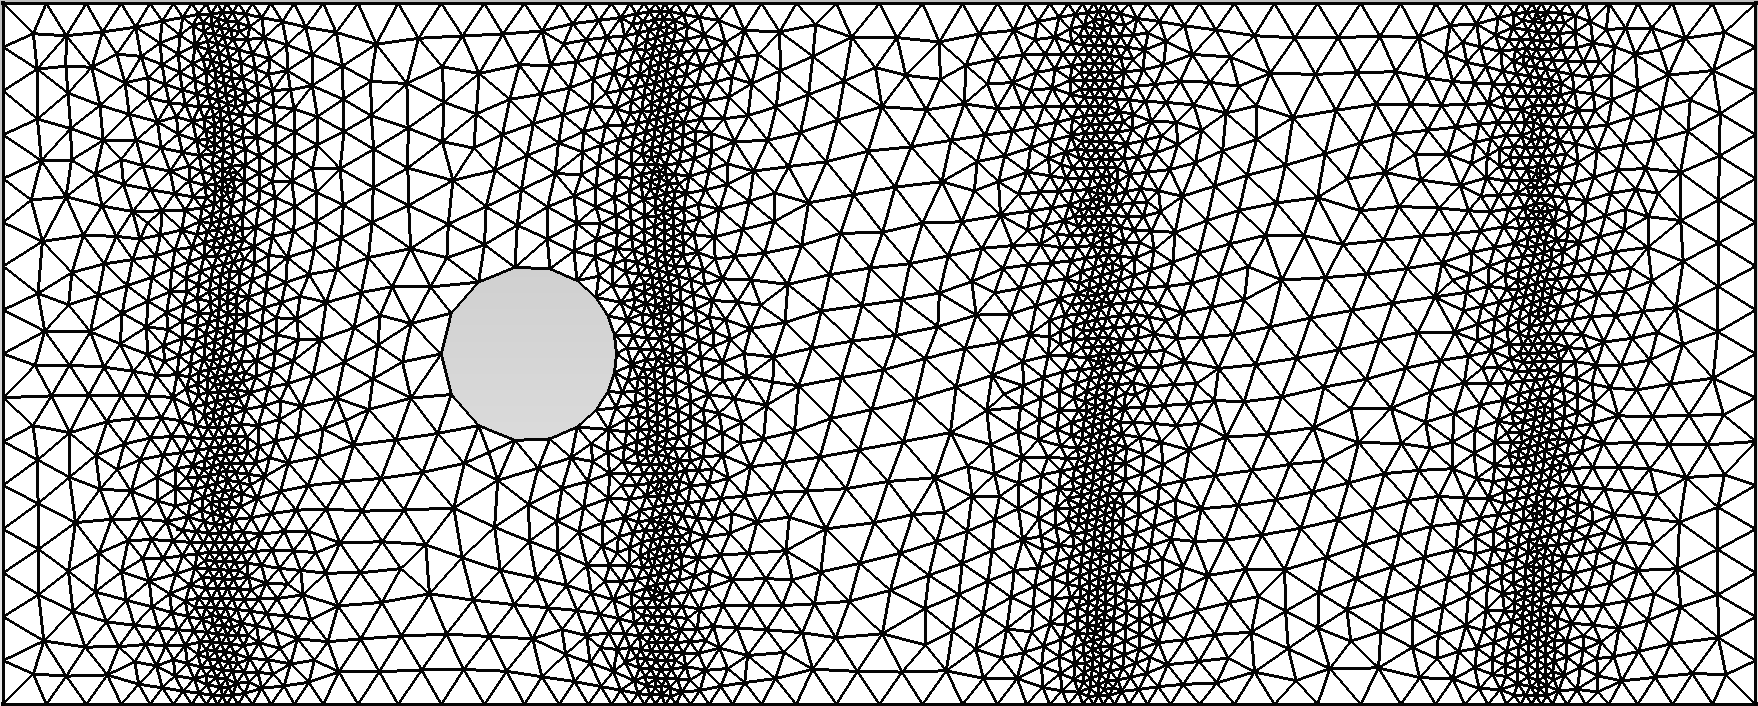
\includegraphics[width=1.02\textwidth]{figures/cosBW.png}
      \caption{}
      \label{}
    \end{figure}
    \vspace{-0.8cm}
    \begin{figure}
      \text{~~~}
      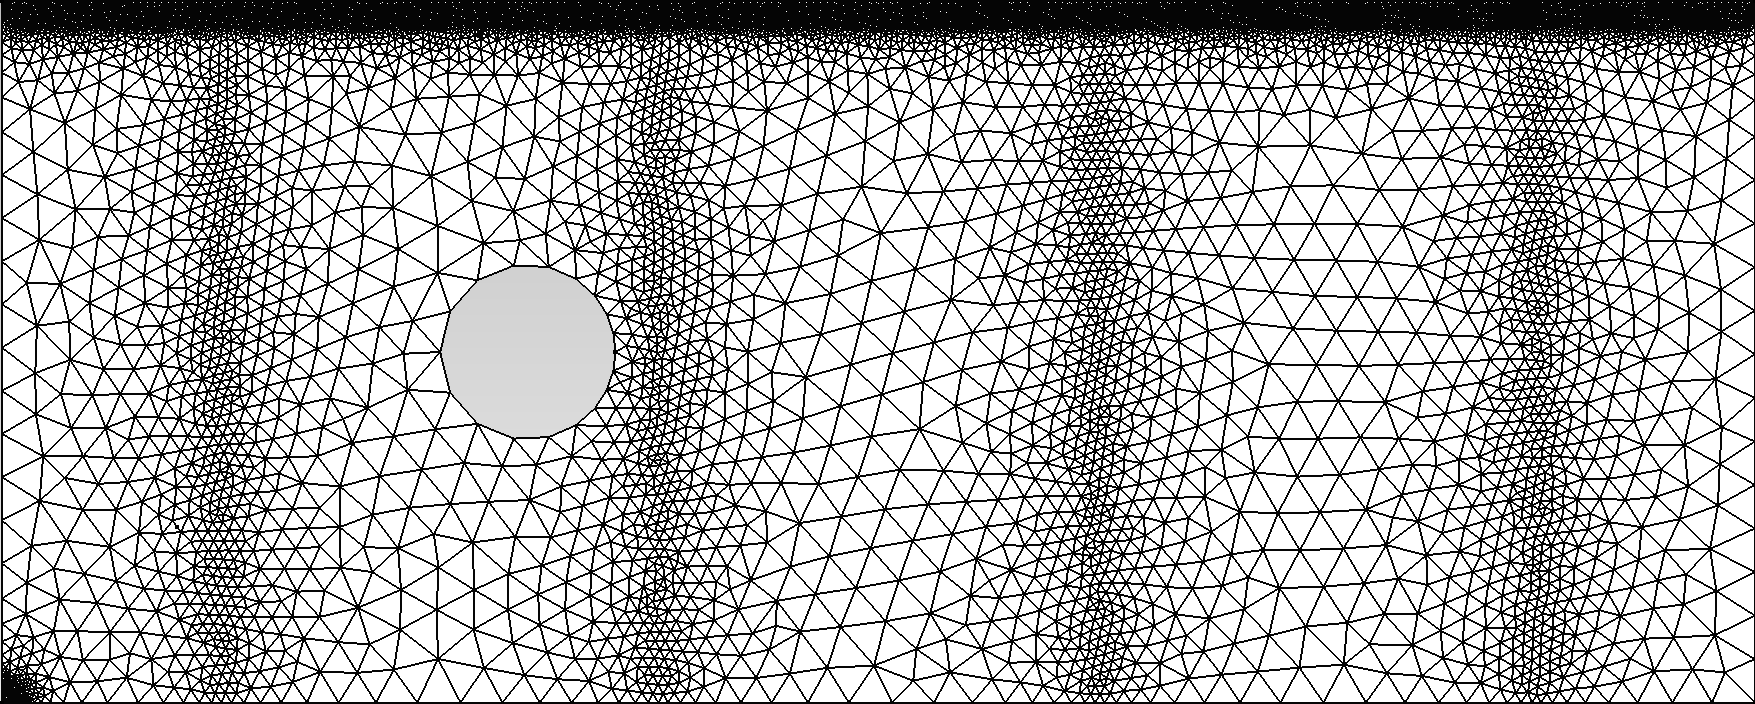
\includegraphics[width=1.02\textwidth]{figures/min.png}
      \caption{}
      \label{}
    \end{figure}
  \end{column}
\end{columns}
\end{frame}

\begin{frame}[fragile]
\frametitle{Champs de taille}
\begin{columns}
  \begin{column}{0.55\textwidth}
    \footnotesize
    \textbf{AutomaticMeshSizeField} : Carte de taille automatique basée sur la courbure et la proximité des bords du CAD. Les tailles calculées aux bords sont propagées à l'intérieur suivant la gradation imposée. Requiert un maillage uniforme raisonnablement fin en entrée.
    \begin{lstlisting}[frame=none]
    // Importe un maillage dans le modele
    Merge "mesh.msh";

    Field[5] = AutomaticMeshSizeField;
    Field[5].nPointsPerCircle = 20;
    Field[5].nPointsPerGap = 25;
    Field[5].gradation = 1.1;
    \end{lstlisting}
  \end{column}
  \begin{column}{0.4\textwidth}
    \vspace{-0.7cm}
    \begin{figure}
      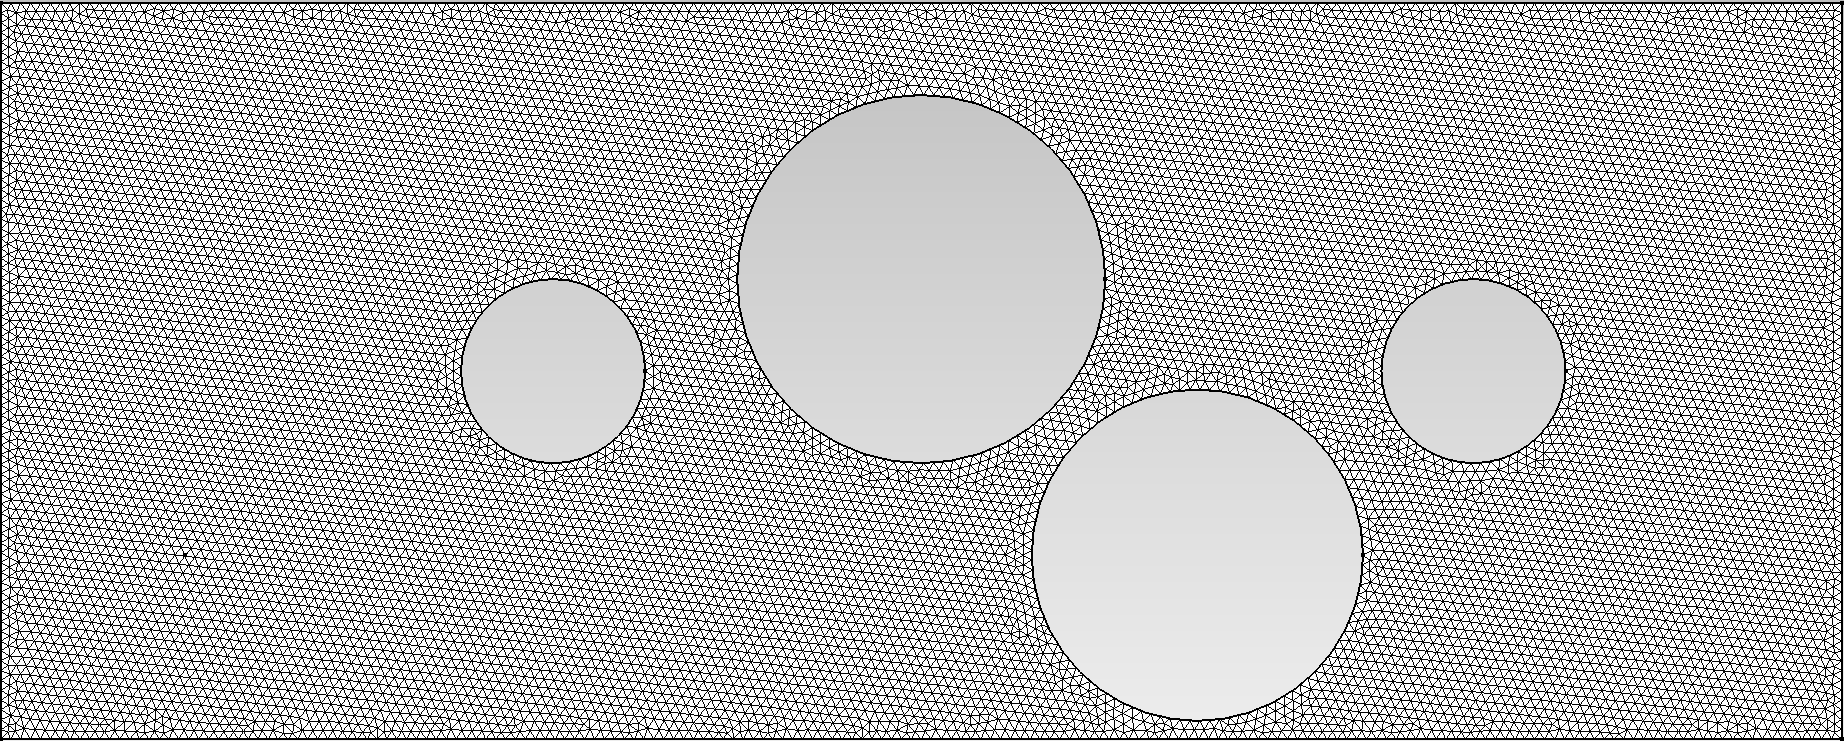
\includegraphics[width=1.02\textwidth]{figures/uniform.png}
      \caption{}
    \end{figure}
    \vspace{-2.3cm}
    \begin{figure}
      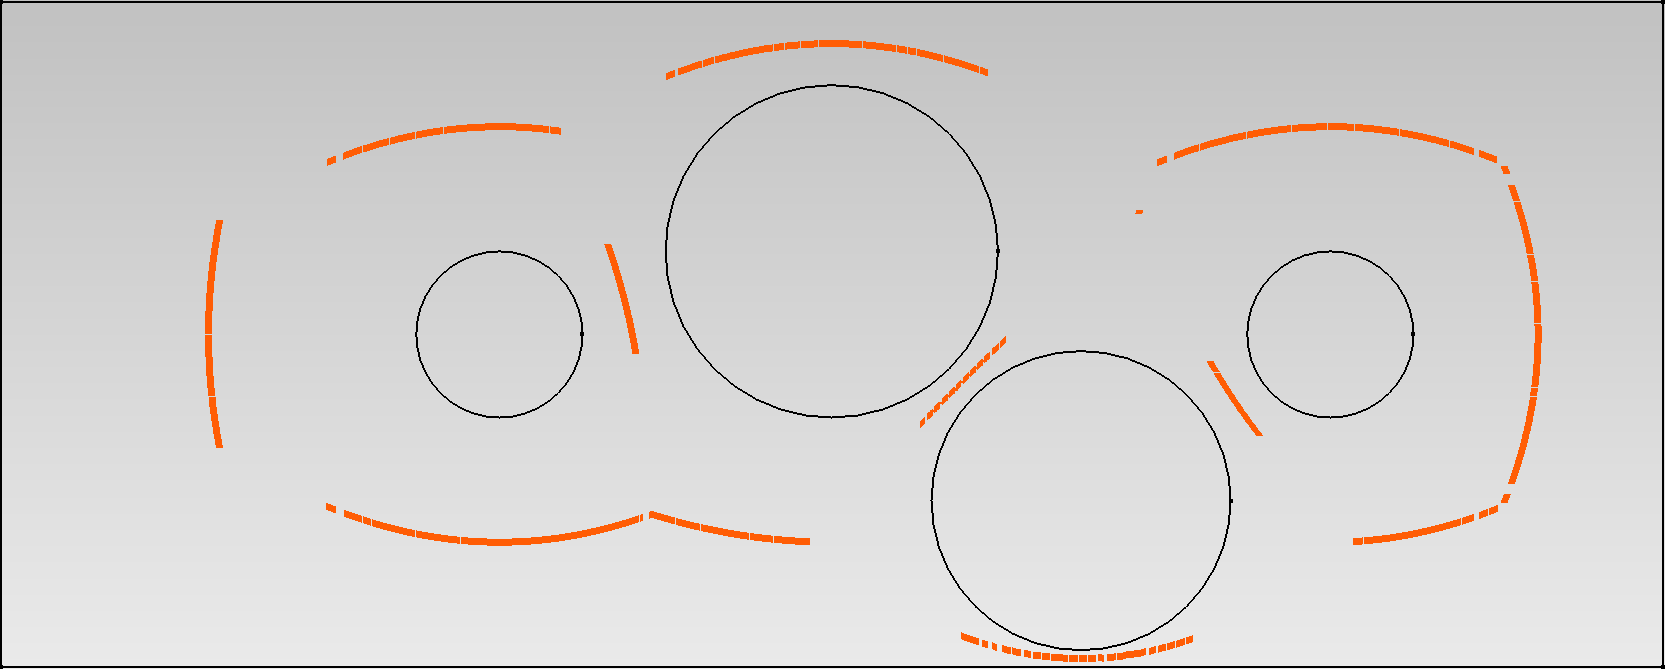
\includegraphics[width=1.02\textwidth]{figures/skeleton.png}
      \caption{}
    \end{figure}
    \vspace{-2.3cm}
    \begin{figure}
      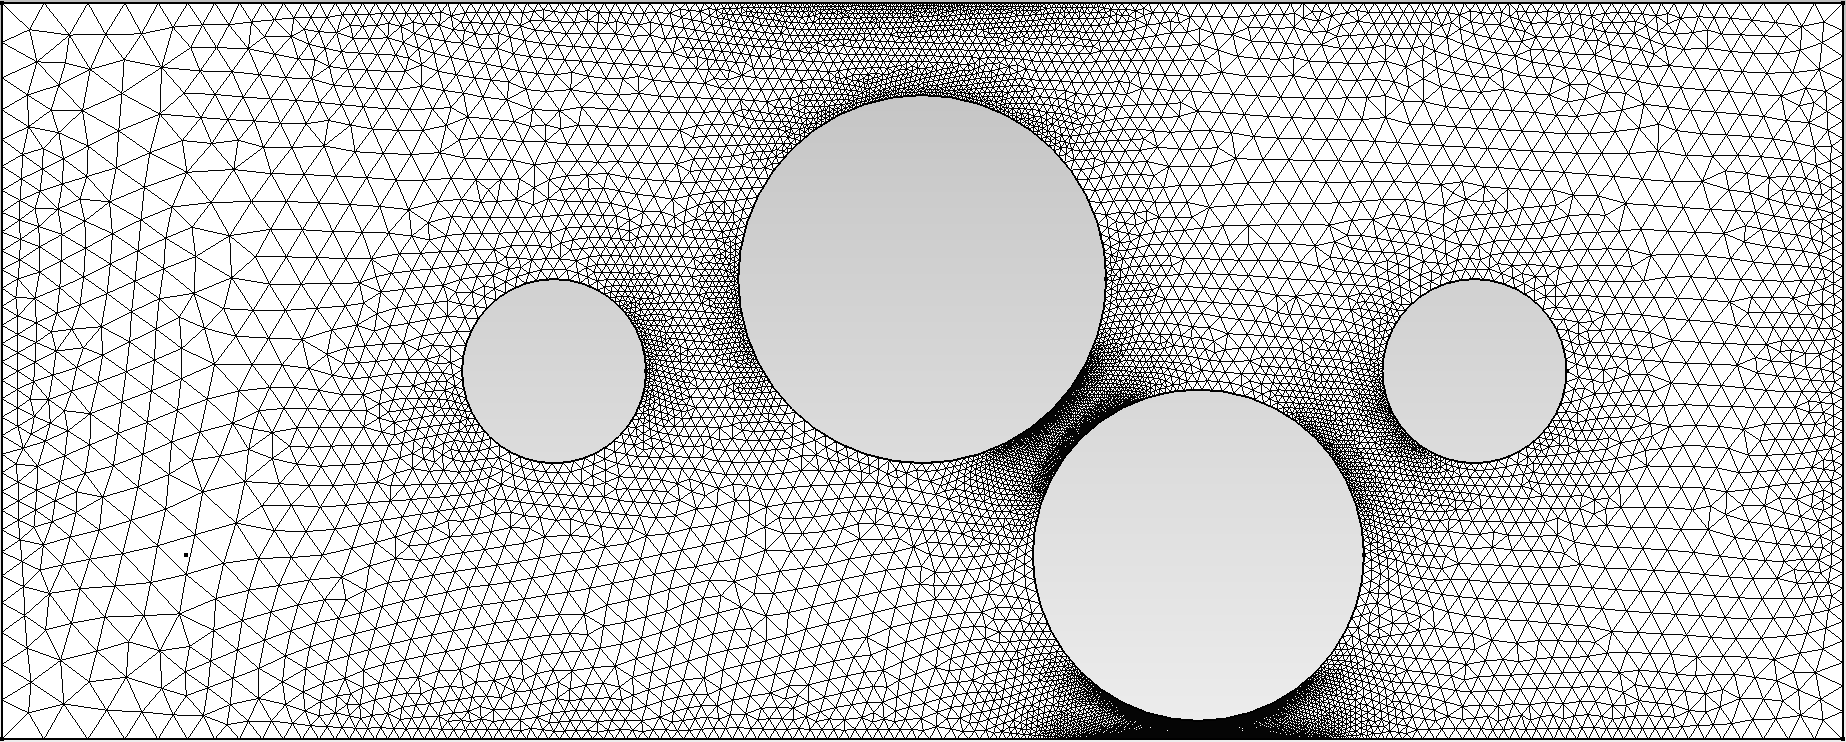
\includegraphics[width=1.02\textwidth]{figures/automatic.png}
      \caption{}
    \end{figure}
  \end{column}
\end{columns}
\footnotetext[1]{Text}
\end{frame}

\begin{frame}[fragile]
\frametitle{Champs de taille \hfill T10}
Finalement :
\begin{lstlisting}[belowskip=0.5mm]
// min(Threshold, MathEval)
Field[4] = Min;
Field[4].FieldsList = {1,2};
// Pour eviter des tailles parasites des frontieres
Mesh.MeshSizeFromPoints = 0;
Mesh.MeshSizeFromCurvature = 0;
Mesh.MeshSizeExtendFromBoundary = 0;
// Applique le champ Min comme carte de taille : indispensable
Background Field = 4;
\end{lstlisting}
\begin{itemize}
  \item Possible de définir des champs depuis l'interface graphique (un peu fastidieux...)
  \item Autres champs disponibles : Box, BoundaryLayer, PostView, ... (voir doc !)
\end{itemize}
\end{frame}

\begin{frame}[fragile]
\frametitle{Générer le maillage}
Dans l'interface graphique :
\begin{enumerate}
  \item File $\rightarrow$ Open $\rightarrow$ foo.geo
  \item Mesh $\rightarrow$ 1D/2D/3D ou simplement "1"/"2"/"3"
\end{enumerate}
En ligne de commande :
\begin{lstlisting}[frame=none, aboveskip=1mm, belowskip=0mm]
gmsh foo.geo -1/-2/-3 // Maillage 1D/2D/3D avec output dans "foo.msh"
\end{lstlisting}
Quelques options :
\begin{lstlisting}[frame=non,aboveskip=1mm,belowskip=0.5mm]
-o [fileName] // Nom du maillage de sortie
-format [msh, msh2, msh4, mesh, inp, ...] // Format du maillage de sortie
-algo [del2d, front2d, delquad, del3d, hxt, ...] // Algorithme de maillage 2D/3D
-order [n] // Ordre des elements
-clscale [val] // Facteur global pour la taille de maille (MeshSizeFactor)
-clmin/-clmax [val] // Taille min/max avant application de MeshSizeFactor
-bgm [fileName] // Charge une carte de taille depuis un fichier (Background Mesh)
-size_field [nodesPer2Pi nodesPerGap gradation] // Carte de taille automatique
\end{lstlisting}
\end{frame}

\begin{frame}[fragile]
\frametitle{Exemples d'appels}
\begin{lstlisting}[frame=none, aboveskip=1mm, belowskip=2mm, escapechar=ß]
// Genere un maillage de triangles de la geometrie decrite dans foo.geo et sauve au format msh4
gmsh foo.geo -2 -o mesh.msh4
// Genere un maillage de tetraedres d'ordre 2 (10 noeuds) avec l'algorithme HXT (reimplementation efficace et parallele du Delaunay 3D) et sauve au format Medit
gmsh foo.geo -3 -order 2 -algo hxt -o mesh.mesh
// Genere un maillage de triangles avec un facteur 0.1 sur la taille decrite dans foo.geo et une taille minimum de 0.01, puis sauve au format msh4 (defaut)
gmsh foo.geo -2 -clscale 0.1 -clmin 1e-2 -o mesh.msh
// Genere un maillage fin uniforme, puis calcule une carte de taille a l'aide du champ AutomaticMeshSizeFieldß\footnote{Requiert que Gmsh soit compil\'e avec la bibliotheque p4est.}ß et l'exporte dans un octree au format .p4est. Ensuite, charge la carte de taille comme maillage de fond avec l'option bgm et maille la geometrie initiale.
gmsh foo.geo -2 -clscale 0.05 -o fooUniform.msh
gmsh fooUniform.msh -size_field 4 20 1.1
gmsh foo.geo -2 -bgm fooUniform.p4est -o mesh.msh
\end{lstlisting}
\end{frame}

\subsection{... via l'API C/C++/Python}

\begin{frame}[fragile]
\frametitle{Créer la géométrie via l'API C++ \hfill t1.cpp}
  \footnotesize
  \begin{lstlisting}[]
  #include <gmsh.h>
  int main(int argc, char **argv)
  {
    gmsh::initialize();
    gmsh::model::add("myBeautifulModel");
    double lc = 0.2, xc = 3., yc = 2., r = 0.5;
    // Points
    gmsh::model::occ::addPoint( 0, 0, 0, lc, 1);
    gmsh::model::occ::addPoint(10, 0, 0, lc, 2);
    gmsh::model::occ::addPoint(10, 4, 0, lc, 3);
    gmsh::model::occ::addPoint( 0, 4, 0, lc, 4);
    // Courbes : un nouveau tag est renvoye si aucun n'est specifie
    int l1 = gmsh::model::occ::addLine(1, 2);
    int l2 = gmsh::model::occ::addLine(2, 3);
    int l3 = gmsh::model::occ::addLine(3, 4);
    int l4 = gmsh::model::occ::addLine(4, 1);
    int c1 = gmsh::model::occ::addCircle(xc, yc, 0, r);
  \end{lstlisting}
\end{frame}

\begin{frame}[fragile]
\frametitle{Créer la géométrie via l'API C++ \hfill t1.cpp}
  \footnotesize
  \begin{lstlisting}[]
    // Curve loops
    int boundary = gmsh::model::occ:addCurveLoop({l1,l2,l3,l4});
    int circle = gmsh::model::occ:addCurveLoop({c1});
    // Surface
    gmsh::model::occ::addPlaneSurface({boundary, circle}, 1);
    // Creation des structures Gmsh associees a la geometrie
    gmsh::model::occ::synchronize();
  }
  \end{lstlisting}
\end{frame}

\end{document}
